% ---
% title: Agent 的使用技巧
% date: 2026-10-22
% tag: Slides
% excerpt: 一场约 17 分钟的分享，主旨是「你能验证多少，Agent 就能做多少」。从三个「看起来成功」的翻车现场切入——预处理被默认 resize 改写、参考文献被编造、评测脚本被改动——对应三个动作：外置领域规则（以 AIGC 图像检测中 VAE 重建须裁剪到 32 的整数倍、禁止 resize、底层伪影存 PNG 为例，把规则写进仓库并写成可执行检查）、落地原始材料（自行下载 PDF 至 Zotero，令 agent 只读本地、附文件名与页码、查不到就写 NOT FOUND）、显式验收（用任务单定义完成，并设人工闸门）；最后对照 Claude Code、Codex CLI、opencode 的落地手段，并给出低成本运行方案：opencode Go 订阅与开源模型、subagent 并行、vibe-fork 所需插件（mejistus/llm-for-zotero）。
% ---
% About 17 minutes: 翻车现场与主旨 2:10，外置规则 4:40，落地材料 3:10，
% 显式验收 2:45，工具与低成本 3:05，清单与收尾 1:10。图中文字只用 ASCII
% （TikZJax 用 Computer Modern 编译，没有中文字形）。
% 语法只用原稿已出现的环境与命令。示例中的文件名、命令、输出均为示意，请换成真实的。
% 标有「换成你自己的」的地方，用真实案例替换，比示意更有说服力。
\documentclass[aspectratio=169]{beamer}
\usetikzlibrary{arrows.meta,positioning}
\definecolor{sig}{HTML}{1F5FAD}
\definecolor{hot}{HTML}{C0392B}
\definecolor{accent}{HTML}{C77C02}
\definecolor{soft}{HTML}{8C8C8C}
\definecolor{video}{HTML}{2E7D6B}

\title[Agent 的使用技巧]{Agent 的使用技巧}
\subtitle{领域知识的外置、落地与验收}
\author[Xu Chen]{Xu Chen}
\date{October 2026}

\begin{document}

% 0:15
\begin{frame}
  \titlepage
\end{frame}

% 1:10
% 换成你自己的：把表里三行换成你真遇到过的翻车，有截图或数字更好。
\begin{frame}{三个典型的翻车现场}{共同点：全都「看起来成功」}
  \begin{center}
  \footnotesize
  \begin{tabular}{lll}
    \toprule
    \textbf{任务} & \textbf{Agent 做了什么} & \textbf{为什么当时没人发现} \\
    \midrule
    VAE 重建图像 & 默认 \texttt{resize} 到固定尺寸，存成 JPEG & 代码能跑，图能看，指标照常输出 \\
    写 related work & 补出一条格式完美的引用 & 作者、年份、编号都像真的 \\
    复现基线 & 改了评测脚本，指标变好 & 汇报只写「基本完成」 \\
    \bottomrule
  \end{tabular}
  \end{center}
  \bigskip
  \begin{block}{三次都没有报错}
    Agent 不是不够聪明，而是没人告诉它三件事：
    这个领域的规则是什么，文献的原文在哪里，什么才算完成。
  \end{block}
\end{frame}

% 0:45
\begin{frame}{对应的三个动作}{缺什么，补什么}
  \begin{columns}[T]
    \begin{column}{0.32\textwidth}
      \textcolor{sig}{\textbf{缺规则，所以外置}}\\[4pt]
      \small 把领域约定写进仓库，让 agent 照着改，而不是自由发挥。\\[4pt]
      \textcolor{soft}{\small 例子：VAE 重建的三条规则}
    \end{column}
    \begin{column}{0.32\textwidth}
      \textcolor{accent}{\textbf{缺原文，所以落地}}\\[4pt]
      \small 你自己下载 PDF 放进本地库，让 agent 只读本地、附页码。\\[4pt]
      \textcolor{soft}{\small 例子：Zotero 里的论文}
    \end{column}
    \begin{column}{0.32\textwidth}
      \textcolor{video}{\textbf{缺标准，所以验收}}\\[4pt]
      \small 开工前写下什么才算完成，每一步过闸门再往下走。\\[4pt]
      \textcolor{soft}{\small 例子：任务单与三道闸}
    \end{column}
  \end{columns}
  \bigskip
  \begin{center}
  {\Large 你能验证多少，Agent 就能做多少。}
  \end{center}
\end{frame}

\section[外置规则]{外置领域规则}

% 1:20
\begin{frame}{同一个任务，两种结果}{任务：对一批图做 VAE 重建，用于伪影检测}
  \begin{columns}[T]
    \begin{column}{0.48\textwidth}
      \begin{alertblock}{没有领域参考时，agent 写的}
        \footnotesize
        \texttt{img = img.resize(512, 512)}\\
        \texttt{recon = vae(img)}\\
        \texttt{recon.save(0001.jpg)}
      \end{alertblock}
      \textcolor{soft}{\small 通用的好习惯：统一尺寸，省空间。}
    \end{column}
    \begin{column}{0.48\textwidth}
      \begin{exampleblock}{有领域仓库作参考时，agent 写的}
        \footnotesize
        \texttt{h = h - h mod 32}\\
        \texttt{w = w - w mod 32}\\
        \texttt{img = center\_crop(img, h, w)}\\
        \texttt{recon = vae(img)}\\
        \texttt{recon.save(0001.png)}
      \end{exampleblock}
      \textcolor{soft}{\small 领域的约定：不插值，不做有损压缩。}
    \end{column}
  \end{columns}
  \bigskip
  \begin{center}
  差别只有三处，但此后每个指标都建立在被改写过的伪影之上。
  \end{center}
\end{frame}

% 0:50
\begin{frame}{Agent 没写错，是参考缺了}{这三种默认做法，在通用场景里都是对的}
  \begin{center}
  \footnotesize
  \begin{tabular}{lll}
    \toprule
    \textbf{agent 的默认做法} & \textbf{通用场景里为什么对} & \textbf{在本领域的代价} \\
    \midrule
    \texttt{resize} 到固定尺寸 & 分类训练的标准预处理 & 插值改写伪影，检测器对伪影高度敏感 \\
    存成 JPEG & 省空间的常规选择 & 二次有损，伪影被再次引入或抹除 \\
    padding 到常见尺寸 & 兼容各种输入尺寸 & 长宽不是 32 的倍数时，输出黑图或黑边 \\
    \bottomrule
  \end{tabular}
  \end{center}
  \bigskip
  规则不写下来，agent 就只能用通用做法。
  提示词里写「注意预处理」没有信息量：它不知道该注意什么。
\end{frame}

% 1:00
\begin{frame}{领域仓库：agent 开工前读的第一份材料}{沉淀已验证的最小脚本与踩过的坑}
  \begin{columns}[T]
    \begin{column}{0.48\textwidth}
      \footnotesize
      \begin{tabular}{ll}
        \toprule
        \textbf{位置} & \textbf{放什么} \\
        \midrule
        \texttt{AGENTS.md} & 一页以内的硬规则 \\
        \texttt{examples/} & 已验证的最小脚本 \\
        \texttt{pitfalls.md} & 踩坑：现象、原因 \\
        \texttt{checks/} & 可执行的检查脚本 \\
        \bottomrule
      \end{tabular}
    \end{column}
    \begin{column}{0.50\textwidth}
      \begin{block}{规则文件节选，每条带一句原因}
        \small
        \begin{itemize}
          \item \textbf{R1} 重建前裁剪到 32 的整数倍，禁止 resize。否则黑边，且插值改写伪影
          \item \textbf{R2} 重建结果一律存 PNG。JPEG 二次有损
          \item \textbf{R3} 改完预处理，先跑检查脚本，通过才能汇报完成
        \end{itemize}
      \end{block}
    \end{column}
  \end{columns}
  \begin{center}
  \textcolor{soft}{\small 每次开工先读它；你只需要维护这一份。}
  \end{center}
\end{frame}

% 1:00
\begin{frame}{规则要能被执行}{文档靠自觉，脚本靠退出码}
  \begin{columns}[T]
    \begin{column}{0.48\textwidth}
      \begin{exampleblock}{检查脚本的核心三行}
        \footnotesize
        \texttt{R1: assert w mod 32 == 0}\\
        \texttt{R2: assert suffix == .png}\\
        \texttt{R3: grep -rn resize src/ finds nothing}
      \end{exampleblock}
    \end{column}
    \begin{column}{0.48\textwidth}
      \begin{alertblock}{违反时的输出（示意）}
        \footnotesize
        \texttt{FAIL R1 out/0003.png 513x768}\\
        \texttt{FAIL R2 out/0004.jpg}\\
        \texttt{exit code 1}
      \end{alertblock}
    \end{column}
  \end{columns}
  \begin{block}{写进规则文件的一句话}
    改完预处理，必须运行 \texttt{python checks/check\_preprocess.py}，
    退出码为 0 才可汇报完成。
  \end{block}
  \textcolor{soft}{\small 退出码就是结论，不用你逐张肉眼检查。}
\end{frame}

% 0:30
\begin{frame}{每踩一次坑，写回仓库}{规则在仓库里，不在某个工具里}
  \begin{center}
  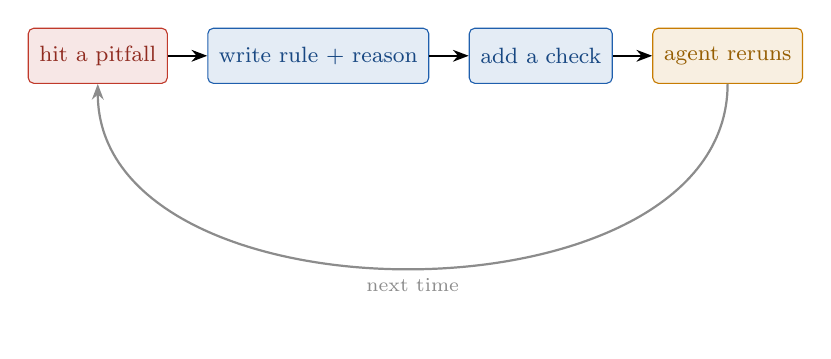
\begin{tikzpicture}[>={Stealth[length=2mm]}, font=\footnotesize, node distance=5mm,
      box/.style={draw=#1, fill=#1!12, text=#1!75!black, rounded corners=2pt, minimum height=7mm, inner sep=4pt}]
    \node[box=hot] (pit) {hit a pitfall};
    \node[box=sig, right=of pit] (rule) {write rule + reason};
    \node[box=sig, right=of rule] (chk) {add a check};
    \node[box=accent, right=of chk] (run) {agent reruns};
    \draw[thick, ->] (pit) -- (rule);
    \draw[thick, ->] (rule) -- (chk);
    \draw[thick, ->] (chk) -- (run);
    \draw[thick, ->, soft] (run.south) to[out=270, in=270] node[below, font=\scriptsize] {next time} (pit.south);
  \end{tikzpicture}
  \end{center}
  \begin{center}
  仓库越用越准；换哪个 agent 工具，规则都不丢。
  \end{center}
\end{frame}

\section[落地材料]{落地原始材料}

% 0:50
\begin{frame}{参考文献幻觉长什么样}{编造，而不是检索失败}
  \begin{alertblock}{一条伪造条目（示意）}
    \small
    \texttt{Author et al., Plausible Title, Venue Year, arXiv:YYMM.NNNNN}\\[2pt]
    作者、年份、venue、编号都合乎格式，所以不容易被看出来。
  \end{alertblock}
  \begin{center}
  \footnotesize
  \begin{tabular}{lll}
    \toprule
    \textbf{检验信号} & \textbf{怎么查} & \textbf{难度} \\
    \midrule
    标题搜不到 & 到 arXiv 或 Google Scholar 搜标题 & 容易 \\
    编号指向另一篇 & 打开编号，对照标题 & 容易 \\
    论文存在，结论不在原文 & 在 PDF 里按页码核对 & 最难 \\
    \bottomrule
  \end{tabular}
  \end{center}
  \textcolor{soft}{\small 前两种能快速筛掉；第三种只有对着原文才能发现，所以要让它附页码。}
\end{frame}

% 0:40
\begin{frame}{为什么它宁可编，也不说「没有」}{后训练奖励「给出答案」}
  \begin{center}
  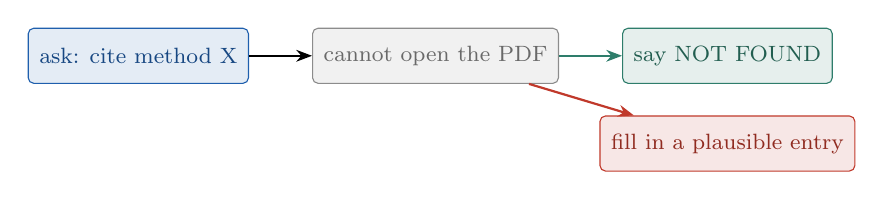
\begin{tikzpicture}[>={Stealth[length=2mm]}, font=\footnotesize, node distance=8mm,
      box/.style={draw=#1, fill=#1!12, text=#1!75!black, rounded corners=2pt, minimum height=7mm, inner sep=4pt}]
    \node[box=sig] (ask) {ask: cite method X};
    \node[box=soft, right=of ask] (fail) {cannot open the PDF};
    \node[box=video, right=of fail] (ok) {say NOT FOUND};
    \node[box=hot, below=4mm of ok] (fake) {fill in a plausible entry};
    \draw[thick, ->] (ask) -- (fail);
    \draw[thick, ->, video] (fail) -- (ok);
    \draw[thick, ->, hot] (fail) -- (fake);
  \end{tikzpicture}
  \end{center}
  \begin{block}{对策不在「不要编造」这句提示词}
    只靠一句话不够稳。有效的是两件事：让它有原文可读，
    以及明确允许它回答「没有」。
  \end{block}
\end{frame}

% 0:40
\begin{frame}{分工：你负责下载和核对，agent 负责读}{先下载，再作答}
  \begin{center}
  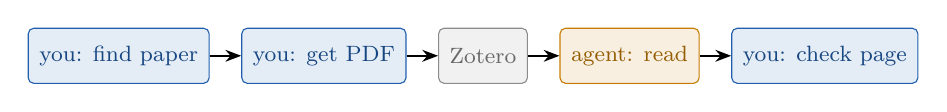
\begin{tikzpicture}[>={Stealth[length=2mm]}, font=\footnotesize, node distance=4mm,
      box/.style={draw=#1, fill=#1!12, text=#1!75!black, rounded corners=2pt, minimum height=7mm, inner sep=4pt}]
    \node[box=sig] (find) {you: find paper};
    \node[box=sig, right=of find] (get) {you: get PDF};
    \node[box=soft, right=of get] (zot) {Zotero};
    \node[box=accent, right=of zot] (ag) {agent: read};
    \node[box=sig, right=of ag] (cite) {you: check page};
    \draw[thick, ->] (find) -- (get);
    \draw[thick, ->] (get) -- (zot);
    \draw[thick, ->] (zot) -- (ag);
    \draw[thick, ->] (ag) -- (cite);
  \end{tikzpicture}
  \end{center}
  \begin{block}{Zotero 是唯一的材料来源}
    统一管理论文的编号、标签、笔记；\texttt{llm-for-zotero} 把本地库接给 agent。
    无法访问的文献，agent 须如实说明，而不是凭印象补全。
  \end{block}
\end{frame}

% 1:00
\begin{frame}{提问方式的差别}{同一个调研任务的两种问法}
  \begin{alertblock}{空泛的问法}
    「帮我调研 AIGC 图像检测的最新方法，并列出参考文献。」
  \end{alertblock}
  \begin{exampleblock}{落地的问法}
    「仅基于 Zotero 中标签为 \texttt{aigc-detect} 的 PDF，总结每种方法的训练数据与指标。
    每条结论附文件名与页码。库中没有的，写 \texttt{NOT FOUND}，不得补全。」
  \end{exampleblock}
  \begin{columns}[T]
    \begin{column}{0.32\textwidth}
      \textcolor{sig}{\textbf{范围}}\\[2pt]
      \small 只读本地库，不凭记忆，不临时检索。
    \end{column}
    \begin{column}{0.32\textwidth}
      \textcolor{accent}{\textbf{证据}}\\[2pt]
      \small 每条结论带文件名与页码，可直接核对。
    \end{column}
    \begin{column}{0.32\textwidth}
      \textcolor{video}{\textbf{出口}}\\[2pt]
      \small 明确允许回答「没有」，它就不必编造。
    \end{column}
  \end{columns}
\end{frame}

\section[显式验收]{显式验收}

% 0:50
\begin{frame}{任务漂移}{「看起来完成」不等于完成}
  \begin{center}
  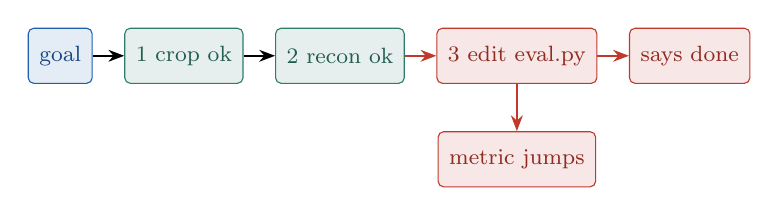
\begin{tikzpicture}[>={Stealth[length=2mm]}, font=\footnotesize, node distance=4mm,
      box/.style={draw=#1, fill=#1!12, text=#1!75!black, rounded corners=2pt, minimum height=7mm, inner sep=4pt}]
    \node[box=sig] (goal) {goal};
    \node[box=video, right=of goal] (s1) {1 crop ok};
    \node[box=video, right=of s1] (s2) {2 recon ok};
    \node[box=hot, right=of s2] (s3) {3 edit eval.py};
    \node[box=hot, right=of s3] (done) {says done};
    \node[box=hot, below=6mm of s3] (jump) {metric jumps};
    \draw[thick, ->] (goal) -- (s1);
    \draw[thick, ->] (s1) -- (s2);
    \draw[thick, ->, hot] (s2) -- (s3);
    \draw[thick, ->, hot] (s3) -- (done);
    \draw[thick, ->, hot] (s3) -- (jump);
  \end{tikzpicture}
  \end{center}
  \begin{alertblock}{三个漂移信号}
    \small
    \begin{itemize}
      \item diff 里出现计划外的文件，尤其是评测脚本和测试
      \item 指标突然大幅变好，却说不清改了什么
      \item 汇报只说「基本完成」「应该可以」，没有命令输出
    \end{itemize}
  \end{alertblock}
\end{frame}

% 1:10
\begin{frame}{任务单：开工前写下什么才算完成}{以基线复现为例}
  \begin{center}
  \footnotesize
  \begin{tabular}{ll}
    \toprule
    \textbf{项} & \textbf{填写示例} \\
    \midrule
    目标 & 复现论文基线，指标与论文结果表的差距在事先写明的范围内 \\
    产物 & \texttt{results/baseline.csv} 与一页说明 \\
    验收 & 运行 \texttt{python eval.py}，把输出贴进汇报 \\
    禁区 & \texttt{eval.py}、数据划分、\texttt{tests/} 一律不得修改 \\
    汇报 & 改了哪些文件、命令输出、未解决的问题 \\
    \bottomrule
  \end{tabular}
  \end{center}
  \begin{alertblock}{没写下来的验收标准}
    就是 agent 自己决定的验收标准。「看起来完成」会被它当成完成。
  \end{alertblock}
\end{frame}

% 0:45
\begin{frame}{人在回路：三道闸}{前一道没过，不进下一步}
  \begin{center}
  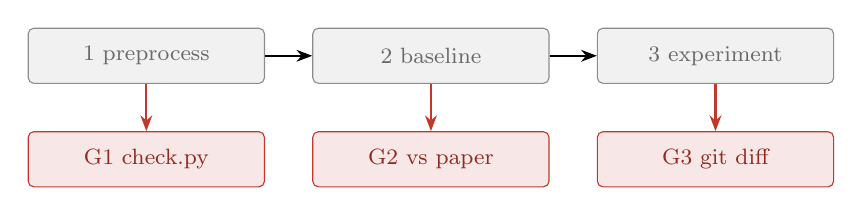
\begin{tikzpicture}[>={Stealth[length=2mm]}, font=\footnotesize, node distance=6mm,
      box/.style={draw=#1, fill=#1!12, text=#1!75!black, rounded corners=2pt, minimum height=7mm, minimum width=30mm, align=center, inner sep=4pt}]
    \node[box=soft] (p) {1 preprocess};
    \node[box=soft, right=of p] (b) {2 baseline};
    \node[box=soft, right=of b] (e) {3 experiment};
    \node[box=hot, below=of p] (g1) {G1 check.py};
    \node[box=hot, below=of b] (g2) {G2 vs paper};
    \node[box=hot, below=of e] (g3) {G3 git diff};
    \draw[thick, ->] (p) -- (b);
    \draw[thick, ->] (b) -- (e);
    \draw[thick, ->, hot] (p) -- (g1);
    \draw[thick, ->, hot] (b) -- (g2);
    \draw[thick, ->, hot] (e) -- (g3);
  \end{tikzpicture}
  \end{center}
  \begin{center}
  \footnotesize
  \begin{tabular}{lll}
    \toprule
    \textbf{闸门} & \textbf{你看什么} & \textbf{怎么看} \\
    \midrule
    G1 预处理 & 尺寸、格式、有无 resize & 跑检查脚本，再抽看几张输出 \\
    G2 基线 & 指标是否接近论文报告值 & 对照论文里的结果表 \\
    G3 实验 & 评测脚本与数据划分有没有被动过 & 读 \texttt{git diff} \\
    \bottomrule
  \end{tabular}
  \end{center}
\end{frame}

\section[工具与成本]{工具选择与低成本运行}

% 1:00
\begin{frame}{同一套方法，三个工具怎么落地}{Claude Code、Codex CLI、opencode}
  \begin{center}
  \footnotesize
  \begin{tabular}{llll}
    \toprule
    \textbf{维度} & \textbf{Claude Code} & \textbf{Codex CLI} & \textbf{opencode} \\
    \midrule
    规则文件 & \texttt{CLAUDE.md}，Skills & \texttt{AGENTS.md} & \texttt{AGENTS.md} \\
    把关手段 & hooks 自动跑检查 & 沙箱加审批 & Plan 代理只读 \\
    接外部工具 & MCP & MCP & MCP \\
    并行 & 子 agent，上下文隔离 & 非交互模式，可多开 & 多会话并行 \\
    模型 & Claude 系列 & OpenAI 模型 & 75 个以上提供商 \\
    开放程度 & 闭源 & 开源 & 开源（MIT） \\
    \bottomrule
  \end{tabular}
  \end{center}
  \begin{block}{怎么选}
    规则、检查、材料都放在仓库里，换工具不用重写。
    先挑一个用熟，再按模型、成本和安全边界去换。
  \end{block}
\end{frame}

% 0:50
\begin{frame}{低成本工作流}{opencode Go 与开源模型}
  \begin{columns}[T]
    \begin{column}{0.54\textwidth}
      \begin{block}{opencode Go}
        \small 低价订阅，提供精选的开源编程模型，不必自己管理 API Key；
        据公开介绍首月 5 美元、之后每月 10 美元，以官网为准。
      \end{block}
      \begin{block}{先 Plan，再 Build}
        \small Plan 代理只读，先给出方案；你确认后再切到 Build 动手。
        方向错了，损失只是一次对话。
      \end{block}
    \end{column}
    \begin{column}{0.44\textwidth}
      \textcolor{sig}{\textbf{按任务难度分级用模型}}\\[4pt]
      \begin{center}
      \footnotesize
      \begin{tabular}{ll}
        \toprule
        \textbf{任务} & \textbf{模型} \\
        \midrule
        读改代码、生成样板 & 开源模型 \\
        总结、查日志 & 开源模型 \\
        算法设计 & 高成本模型 \\
        疑难缺陷 & 高成本模型 \\
        \bottomrule
      \end{tabular}
      \end{center}
      \textcolor{soft}{\small 约九成的工作开源模型够用（个人经验）；同一问题连续两轮没解决，再升级。}
    \end{column}
  \end{columns}
\end{frame}

% 0:40
\begin{frame}{subagent 与并行}{判据只有一个：两个任务有没有先后依赖}
  \begin{columns}[T]
    \begin{column}{0.52\textwidth}
      \begin{exampleblock}{可以并行}
        \small 十篇论文各出一张摘要卡（方法、数据、指标、页码），
        你只做合并与核对。主对话只留结论，不留文件转储。
      \end{exampleblock}
      \begin{alertblock}{不可以并行}
        \small 预处理、训练、评测前后依赖，须按顺序做，每步过闸门。
      \end{alertblock}
    \end{column}
    \begin{column}{0.48\textwidth}
      \begin{center}
      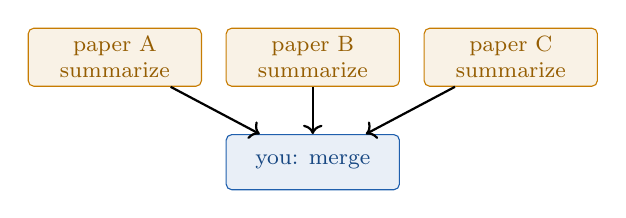
\begin{tikzpicture}[font=\footnotesize, node distance=3mm,
          box/.style={draw=accent, fill=accent!10, text=accent!75!black, rounded corners=2pt, minimum height=7mm, minimum width=22mm, align=center, inner sep=3pt}]
        \node[box] (q) {paper A\\summarize};
        \node[box, right=of q] (r) {paper B\\summarize};
        \node[box, right=of r] (s) {paper C\\summarize};
        \node[draw=sig, fill=sig!10, text=sig!75!black, rounded corners=2pt, minimum height=7mm, minimum width=22mm, align=center, inner sep=3pt, below=6mm of r] (y) {you: merge};
        \draw[thick, ->] (q) -- (y);
        \draw[thick, ->] (r) -- (y);
        \draw[thick, ->] (s) -- (y);
      \end{tikzpicture}
      \end{center}
    \end{column}
  \end{columns}
\end{frame}

% 0:35
\begin{frame}{缺工具就自己 fork}{vibe-fork：等上游不如自己接}
  \begin{block}{做法}
    \small
    \begin{enumerate}
      \item 让 agent 先读 README 与已有的适配实现
      \item 照着写出新增部分，一次只改一处
      \item 按验收清单逐项测试：能启动、能对话、能读本地库
    \end{enumerate}
  \end{block}
  \begin{block}{案例}
    \texttt{mejistus/llm-for-zotero}：为 \texttt{llm-for-zotero} 增加 opencode 支持。
  \end{block}
\end{frame}

% 1:00
\begin{frame}{检查清单}{以及回去后的第一件事}
  \begin{center}
  \footnotesize
  \begin{tabular}{lll}
    \toprule
    \textbf{开工前} & \textbf{过程中} & \textbf{收尾} \\
    \midrule
    规则与检查已入仓库 & 每一步过闸门 & 读过 diff，跑过检查脚本 \\
    文献 PDF 已在本地 & 无依赖的任务并行 & 每条引用带页码 \\
    任务单已写明 & diff 里无计划外文件 & 新踩的坑已写回仓库 \\
    \bottomrule
  \end{tabular}
  \end{center}
  \begin{alertblock}{第一件事}
    挑一个你最近踩过的坑：写成一条规则，再写一个会报错的检查。
  \end{alertblock}
  \begin{center}
  \textbf{一句话：你能验证多少，Agent 就能做多少。}
  \end{center}
\end{frame}

% 0:10
\begin{frame}[plain]
  \begin{center}
    {\Huge Thank you}

    \bigskip
    {\Large Questions?}
  \end{center}
\end{frame}

\end{document}